% Options for packages loaded elsewhere
\PassOptionsToPackage{unicode}{hyperref}
\PassOptionsToPackage{hyphens}{url}
\PassOptionsToPackage{dvipsnames,svgnames,x11names}{xcolor}
%
\documentclass[
  letterpaper,
  DIV=11,
  numbers=noendperiod]{scrartcl}

\usepackage{amsmath,amssymb}
\usepackage{iftex}
\ifPDFTeX
  \usepackage[T1]{fontenc}
  \usepackage[utf8]{inputenc}
  \usepackage{textcomp} % provide euro and other symbols
\else % if luatex or xetex
  \usepackage{unicode-math}
  \defaultfontfeatures{Scale=MatchLowercase}
  \defaultfontfeatures[\rmfamily]{Ligatures=TeX,Scale=1}
\fi
\usepackage{lmodern}
\ifPDFTeX\else  
    % xetex/luatex font selection
\fi
% Use upquote if available, for straight quotes in verbatim environments
\IfFileExists{upquote.sty}{\usepackage{upquote}}{}
\IfFileExists{microtype.sty}{% use microtype if available
  \usepackage[]{microtype}
  \UseMicrotypeSet[protrusion]{basicmath} % disable protrusion for tt fonts
}{}
\makeatletter
\@ifundefined{KOMAClassName}{% if non-KOMA class
  \IfFileExists{parskip.sty}{%
    \usepackage{parskip}
  }{% else
    \setlength{\parindent}{0pt}
    \setlength{\parskip}{6pt plus 2pt minus 1pt}}
}{% if KOMA class
  \KOMAoptions{parskip=half}}
\makeatother
\usepackage{xcolor}
\setlength{\emergencystretch}{3em} % prevent overfull lines
\setcounter{secnumdepth}{-\maxdimen} % remove section numbering
% Make \paragraph and \subparagraph free-standing
\ifx\paragraph\undefined\else
  \let\oldparagraph\paragraph
  \renewcommand{\paragraph}[1]{\oldparagraph{#1}\mbox{}}
\fi
\ifx\subparagraph\undefined\else
  \let\oldsubparagraph\subparagraph
  \renewcommand{\subparagraph}[1]{\oldsubparagraph{#1}\mbox{}}
\fi


\providecommand{\tightlist}{%
  \setlength{\itemsep}{0pt}\setlength{\parskip}{0pt}}\usepackage{longtable,booktabs,array}
\usepackage{calc} % for calculating minipage widths
% Correct order of tables after \paragraph or \subparagraph
\usepackage{etoolbox}
\makeatletter
\patchcmd\longtable{\par}{\if@noskipsec\mbox{}\fi\par}{}{}
\makeatother
% Allow footnotes in longtable head/foot
\IfFileExists{footnotehyper.sty}{\usepackage{footnotehyper}}{\usepackage{footnote}}
\makesavenoteenv{longtable}
\usepackage{graphicx}
\makeatletter
\def\maxwidth{\ifdim\Gin@nat@width>\linewidth\linewidth\else\Gin@nat@width\fi}
\def\maxheight{\ifdim\Gin@nat@height>\textheight\textheight\else\Gin@nat@height\fi}
\makeatother
% Scale images if necessary, so that they will not overflow the page
% margins by default, and it is still possible to overwrite the defaults
% using explicit options in \includegraphics[width, height, ...]{}
\setkeys{Gin}{width=\maxwidth,height=\maxheight,keepaspectratio}
% Set default figure placement to htbp
\makeatletter
\def\fps@figure{htbp}
\makeatother
% definitions for citeproc citations
\NewDocumentCommand\citeproctext{}{}
\NewDocumentCommand\citeproc{mm}{%
  \begingroup\def\citeproctext{#2}\cite{#1}\endgroup}
\makeatletter
 % allow citations to break across lines
 \let\@cite@ofmt\@firstofone
 % avoid brackets around text for \cite:
 \def\@biblabel#1{}
 \def\@cite#1#2{{#1\if@tempswa , #2\fi}}
\makeatother
\newlength{\cslhangindent}
\setlength{\cslhangindent}{1.5em}
\newlength{\csllabelwidth}
\setlength{\csllabelwidth}{3em}
\newenvironment{CSLReferences}[2] % #1 hanging-indent, #2 entry-spacing
 {\begin{list}{}{%
  \setlength{\itemindent}{0pt}
  \setlength{\leftmargin}{0pt}
  \setlength{\parsep}{0pt}
  % turn on hanging indent if param 1 is 1
  \ifodd #1
   \setlength{\leftmargin}{\cslhangindent}
   \setlength{\itemindent}{-1\cslhangindent}
  \fi
  % set entry spacing
  \setlength{\itemsep}{#2\baselineskip}}}
 {\end{list}}
\usepackage{calc}
\newcommand{\CSLBlock}[1]{\hfill\break\parbox[t]{\linewidth}{\strut\ignorespaces#1\strut}}
\newcommand{\CSLLeftMargin}[1]{\parbox[t]{\csllabelwidth}{\strut#1\strut}}
\newcommand{\CSLRightInline}[1]{\parbox[t]{\linewidth - \csllabelwidth}{\strut#1\strut}}
\newcommand{\CSLIndent}[1]{\hspace{\cslhangindent}#1}

\KOMAoption{captions}{tableheading}
\makeatletter
\@ifpackageloaded{caption}{}{\usepackage{caption}}
\AtBeginDocument{%
\ifdefined\contentsname
  \renewcommand*\contentsname{Table of contents}
\else
  \newcommand\contentsname{Table of contents}
\fi
\ifdefined\listfigurename
  \renewcommand*\listfigurename{List of Figures}
\else
  \newcommand\listfigurename{List of Figures}
\fi
\ifdefined\listtablename
  \renewcommand*\listtablename{List of Tables}
\else
  \newcommand\listtablename{List of Tables}
\fi
\ifdefined\figurename
  \renewcommand*\figurename{Figure}
\else
  \newcommand\figurename{Figure}
\fi
\ifdefined\tablename
  \renewcommand*\tablename{Table}
\else
  \newcommand\tablename{Table}
\fi
}
\@ifpackageloaded{float}{}{\usepackage{float}}
\floatstyle{ruled}
\@ifundefined{c@chapter}{\newfloat{codelisting}{h}{lop}}{\newfloat{codelisting}{h}{lop}[chapter]}
\floatname{codelisting}{Listing}
\newcommand*\listoflistings{\listof{codelisting}{List of Listings}}
\makeatother
\makeatletter
\makeatother
\makeatletter
\@ifpackageloaded{caption}{}{\usepackage{caption}}
\@ifpackageloaded{subcaption}{}{\usepackage{subcaption}}
\makeatother
\ifLuaTeX
  \usepackage{selnolig}  % disable illegal ligatures
\fi
\usepackage{bookmark}

\IfFileExists{xurl.sty}{\usepackage{xurl}}{} % add URL line breaks if available
\urlstyle{same} % disable monospaced font for URLs
\hypersetup{
  pdftitle={Predicting Wine Quality Score (Group 18)},
  pdfauthor={Sid Ahuja, Xander Dawson, Zackarya Hamza},
  colorlinks=true,
  linkcolor={blue},
  filecolor={Maroon},
  citecolor={Blue},
  urlcolor={Blue},
  pdfcreator={LaTeX via pandoc}}

\title{Predicting Wine Quality Score (Group 18)}
\author{Sid Ahuja, Xander Dawson, Zackarya Hamza}
\date{}

\begin{document}
\maketitle

\renewcommand*\contentsname{Table of contents}
{
\hypersetup{linkcolor=}
\setcounter{tocdepth}{3}
\tableofcontents
}
\subsection{Summary}\label{summary}

In this report we attempt to build a k-nearest neighbors (k-nn)
classification model which predicts the quality of a Portuguese white
wine based on its chemical components and physical properties. The
dataset classified the wine qualities on a 10-point scale which we
transformed to a binary classification problem where wines with scores
of 0-5 are considered low-quality and scores of 6-10 are considered
high-quality. Our final model had an accuracy of 0.77, correctly
predicting 77\% of the test set samples. It did a better job at
correctly predicting good quality wines than bad quality wines with a
recall score of 0.89. While this model can definitely be improved upon,
the implications of incorrect predictions are not very harmful.
Additionally, it is likely that this model will not be used solely to
make decisions about wine quality and production, but rather be used
alongside with other tools and rankings by professional sommeliers as
well as personal preferences of consumers. With this, we believe this
model can be used to make predictions about Portuguese white wines but
will require further training to be used on other wines.

\subsection{Introduction}\label{introduction}

Portugal is internationally recognized for its exceptional wines and
booming wine industry. This distinction is rooted in the country's rich
viniculture history and its diverse climatic conditions, which
contribute to the production of wines with unique flavors and aromas.
However, with the wine market becoming increasingly saturated and
competitive, the ability to accurately assess the quality of wine based
on objective measurements has become highly valuable. The quality of a
wine is heavily influenced by its various chemical components and
physical properties and such features can be used to predict the quality
of a wine (Fernandes Ferreira Madureira and Simões de Sousa Nunes 2013).

In this report, we aim to explore the application of machine learning
algorithms in predicting the quality of Portuguese white wines, based on
their chemical compositions and physical properties. Our goal is to
develop a predictive model that can distinguish between high and
low-quality wines with a high degree of accuracy. The significance of
such a model lies in its potential to provide consumers with quality
predictions prior to purchase as well as provide produced with
information on ways to improve their wines; our model should be
particularly good at identifying good wines to provide such information
to manufacturers. Through the application of machine learning, this
study contributes to the growing field of data-driven approaches in food
science and quality assurance, marking a step towards the integration of
technology and quality wine production.

\subsection{Methods}\label{methods}

\subsubsection{Data}\label{data}

In order to explore and build a wine quality classification model, we
are using the wine quality data set sourced from the
\href{https://archive.ics.uci.edu/dataset/186/wine+quality}{UCI Machine
Learning Repository} and created by P. Cortez, A. Cerdeira, F. Almeida,
T. Matos and J. Reis from the University of Minho in Portugal (Cortez
and Reis 2009). Specifically, we are interested in predicting white wine
quality based on the chemical composition of the wine. Each row
represents a white wine and the chemical measurements taken from the
wine and there are 4898 samples in the dataset. The target value
(integer wine quality score) was determined by the Vinho Verde Wine
Commission (CVRVV) of Portugal (\emph{Vinho Verde} 2024).

\begin{longtable}[]{@{}
  >{\centering\arraybackslash}p{(\columnwidth - 4\tabcolsep) * \real{0.3333}}
  >{\centering\arraybackslash}p{(\columnwidth - 4\tabcolsep) * \real{0.3333}}
  >{\centering\arraybackslash}p{(\columnwidth - 4\tabcolsep) * \real{0.3333}}@{}}
\caption{Column Descriptions}\label{tbl-cols}\tabularnewline
\toprule\noalign{}
\begin{minipage}[b]{\linewidth}\centering
Feature
\end{minipage} & \begin{minipage}[b]{\linewidth}\centering
Type
\end{minipage} & \begin{minipage}[b]{\linewidth}\centering
Description
\end{minipage} \\
\midrule\noalign{}
\endfirsthead
\toprule\noalign{}
\begin{minipage}[b]{\linewidth}\centering
Feature
\end{minipage} & \begin{minipage}[b]{\linewidth}\centering
Type
\end{minipage} & \begin{minipage}[b]{\linewidth}\centering
Description
\end{minipage} \\
\midrule\noalign{}
\endhead
\bottomrule\noalign{}
\endlastfoot
Fixed Acitity & Coninuous & Concentration (g/L) of tartaric acid.Impacts
the tartness of wines. \\
Volatile Acitity & Coninuous & Concentration (g/L) of acetic
acid.Impacts the vinegar-like taste in wines. \\
Citric Acid & Coninuous & Concentration (g/L) of citric acid.Impacts the
freshness of wines. \\
Residual Sugar & Coninuous & Concentration (g/L) of sugar remaining
after fermentation.Impacts the sweetness of wines. \\
Chlorides & Coninuous & Concentration (g/L) of chlorides.Impacts the
saltiness of wines. \\
Free Sulfur Dioxide & Coninuous & Concentration (mg/L) of unbound
SO2.Prevents microbial growth. \\
Total Sulfur Dioxide & Coninuous & Concentration (mg/L) of total
SO2.Prevents microbial growth and impacts aroma/taste. \\
Density & Coninuous & Density (g/mL) measurement.Relates alcohol to
sugar content. \\
pH & Coninuous & Measurement of wine acidity. \\
Suphates & Coninuous & Concentration (mg/L) of total sulphates. \\
Alcohol & Coninuous & Percentage (\%) of alcohol content. \\
\end{longtable}

\subsubsection{Analysis}\label{analysis}

To predict the wine quality, we utilized the k-nearest neighbors (k-nn)
algorithm and built a classification model based on certain features
within the dataset (specifically alcohol, volatile acidity, total sulfur
dioxide content, density, chlorides, and residual sugar of the wines).
First we converted the quality\_score target column into a
quality\_class column where scores 0-5 were considered bad and scores
6-10 were considered good. We did this to reduce the number of target
classes (creating a binary classification problem) as well as to allow
for more examples within each class. Then we split the data into train
(70\%) and test splits (30\%). All selected features were scaled prior
to model training. We selected the features based on a qualitative
analysis of their distribution for each class; features that greatly
overlapped across classes were dropped. Then, the best value for
hyperparameter K was determined using a 10-fold cross-validation test.
For this model, we determined accuracy to be the best measurement/metric
for assessing our model as there are a similar number of samples within
each class. For the confusion matrix metrics, we consider good to be the
positive category and bad to be the negative category. The R programming
language (R Core Team 2019) and the following packages were used to
perform the analysis: tidyverse (Wickham 2017), tidymodels (Kuhn and
Wickham 2020), repr (Angerer, Kluyver, and Schulz 2023), psych (William
Revelle 2024), kknn (Schliep and Hechenbichler 2016), and knitr(Xie
2014).

\subsection{Results}\label{results}

We start by loading in the raw data as seen in Table~\ref{tbl-raw-data}.
Then we processed the data and generated a summary table describing the
features within the dataset, shown in Table~\ref{tbl-summary-stats}.

\begin{longtable}[]{@{}
  >{\raggedleft\arraybackslash}p{(\columnwidth - 22\tabcolsep) * \real{0.0909}}
  >{\raggedleft\arraybackslash}p{(\columnwidth - 22\tabcolsep) * \real{0.1104}}
  >{\raggedleft\arraybackslash}p{(\columnwidth - 22\tabcolsep) * \real{0.0779}}
  >{\raggedleft\arraybackslash}p{(\columnwidth - 22\tabcolsep) * \real{0.0974}}
  >{\raggedleft\arraybackslash}p{(\columnwidth - 22\tabcolsep) * \real{0.0649}}
  >{\raggedleft\arraybackslash}p{(\columnwidth - 22\tabcolsep) * \real{0.1299}}
  >{\raggedleft\arraybackslash}p{(\columnwidth - 22\tabcolsep) * \real{0.1364}}
  >{\raggedleft\arraybackslash}p{(\columnwidth - 22\tabcolsep) * \real{0.0519}}
  >{\raggedleft\arraybackslash}p{(\columnwidth - 22\tabcolsep) * \real{0.0325}}
  >{\raggedleft\arraybackslash}p{(\columnwidth - 22\tabcolsep) * \real{0.0649}}
  >{\raggedleft\arraybackslash}p{(\columnwidth - 22\tabcolsep) * \real{0.0519}}
  >{\raggedleft\arraybackslash}p{(\columnwidth - 22\tabcolsep) * \real{0.0909}}@{}}

\caption{\label{tbl-raw-data}Raw Wine Data}

\tabularnewline

\toprule\noalign{}
\begin{minipage}[b]{\linewidth}\raggedleft
fixed\_acidity
\end{minipage} & \begin{minipage}[b]{\linewidth}\raggedleft
volatile\_acidity
\end{minipage} & \begin{minipage}[b]{\linewidth}\raggedleft
citric\_acid
\end{minipage} & \begin{minipage}[b]{\linewidth}\raggedleft
residual\_sugar
\end{minipage} & \begin{minipage}[b]{\linewidth}\raggedleft
chlorides
\end{minipage} & \begin{minipage}[b]{\linewidth}\raggedleft
free\_sulfur\_dioxide
\end{minipage} & \begin{minipage}[b]{\linewidth}\raggedleft
total\_sulfur\_dioxide
\end{minipage} & \begin{minipage}[b]{\linewidth}\raggedleft
density
\end{minipage} & \begin{minipage}[b]{\linewidth}\raggedleft
pH
\end{minipage} & \begin{minipage}[b]{\linewidth}\raggedleft
sulphates
\end{minipage} & \begin{minipage}[b]{\linewidth}\raggedleft
alcohol
\end{minipage} & \begin{minipage}[b]{\linewidth}\raggedleft
quality\_score
\end{minipage} \\
\midrule\noalign{}
\endhead
\bottomrule\noalign{}
\endlastfoot
7.0 & 0.27 & 0.36 & 20.7 & 0.045 & 45 & 170 & 1.0010 & 3.00 & 0.45 & 8.8
& 6 \\
6.3 & 0.30 & 0.34 & 1.6 & 0.049 & 14 & 132 & 0.9940 & 3.30 & 0.49 & 9.5
& 6 \\
8.1 & 0.28 & 0.40 & 6.9 & 0.050 & 30 & 97 & 0.9951 & 3.26 & 0.44 & 10.1
& 6 \\
7.2 & 0.23 & 0.32 & 8.5 & 0.058 & 47 & 186 & 0.9956 & 3.19 & 0.40 & 9.9
& 6 \\
7.2 & 0.23 & 0.32 & 8.5 & 0.058 & 47 & 186 & 0.9956 & 3.19 & 0.40 & 9.9
& 6 \\
8.1 & 0.28 & 0.40 & 6.9 & 0.050 & 30 & 97 & 0.9951 & 3.26 & 0.44 & 10.1
& 6 \\

\end{longtable}

\begin{longtable}[]{@{}
  >{\raggedleft\arraybackslash}p{(\columnwidth - 12\tabcolsep) * \real{0.0769}}
  >{\raggedleft\arraybackslash}p{(\columnwidth - 12\tabcolsep) * \real{0.1846}}
  >{\raggedleft\arraybackslash}p{(\columnwidth - 12\tabcolsep) * \real{0.1692}}
  >{\raggedleft\arraybackslash}p{(\columnwidth - 12\tabcolsep) * \real{0.1385}}
  >{\raggedleft\arraybackslash}p{(\columnwidth - 12\tabcolsep) * \real{0.1231}}
  >{\raggedleft\arraybackslash}p{(\columnwidth - 12\tabcolsep) * \real{0.1538}}
  >{\raggedleft\arraybackslash}p{(\columnwidth - 12\tabcolsep) * \real{0.1538}}@{}}

\caption{\label{tbl-summary-stats}Summary statistics of each column in
the dataset}

\tabularnewline

\toprule\noalign{}
\begin{minipage}[b]{\linewidth}\raggedleft
n
\end{minipage} & \begin{minipage}[b]{\linewidth}\raggedleft
mean
\end{minipage} & \begin{minipage}[b]{\linewidth}\raggedleft
sd
\end{minipage} & \begin{minipage}[b]{\linewidth}\raggedleft
median
\end{minipage} & \begin{minipage}[b]{\linewidth}\raggedleft
min
\end{minipage} & \begin{minipage}[b]{\linewidth}\raggedleft
max
\end{minipage} & \begin{minipage}[b]{\linewidth}\raggedleft
range
\end{minipage} \\
\midrule\noalign{}
\endhead
\bottomrule\noalign{}
\endlastfoot
3428 & 6.8647170 & 0.8350113 & 6.8000 & 3.90000 & 14.20000 & 10.30000 \\
3428 & 0.2772943 & 0.0996217 & 0.2600 & 0.08000 & 0.96500 & 0.88500 \\
3428 & 0.3327100 & 0.1176027 & 0.3100 & 0.00000 & 1.00000 & 1.00000 \\
3428 & 6.4113040 & 5.0873601 & 5.3000 & 0.60000 & 65.80000 & 65.20000 \\
3428 & 0.0457611 & 0.0219342 & 0.0430 & 0.00900 & 0.34600 & 0.33700 \\
3428 & 35.3327013 & 17.0846500 & 34.0000 & 2.00000 & 289.00000 &
287.00000 \\
3428 & 138.0439032 & 42.2618066 & 134.0000 & 9.00000 & 440.00000 &
431.00000 \\
3428 & 0.9940724 & 0.0029959 & 0.9938 & 0.98713 & 1.03898 & 0.05185 \\
3428 & 3.1875875 & 0.1502339 & 3.1800 & 2.74000 & 3.81000 & 1.07000 \\
3428 & 0.4889673 & 0.1139145 & 0.4700 & 0.22000 & 1.08000 & 0.86000 \\
3428 & 10.4881145 & 1.2175065 & 10.3000 & 8.00000 & 14.20000 &
6.20000 \\
3428 & 1.6651109 & 0.4720206 & 2.0000 & 1.00000 & 2.00000 & 1.00000 \\

\end{longtable}

We can see in Table~\ref{tbl-summary-stats} that there are no missing
values as well as the summary metrics for each column. This table is
generated using unscaled data so that we can use out intuition and
recall the specific units of each column, gaining a better understanding
of the column characteristics.

\begin{longtable}[]{@{}
  >{\raggedright\arraybackslash}p{(\columnwidth - 26\tabcolsep) * \real{0.0780}}
  >{\raggedleft\arraybackslash}p{(\columnwidth - 26\tabcolsep) * \real{0.0275}}
  >{\raggedleft\arraybackslash}p{(\columnwidth - 26\tabcolsep) * \real{0.0505}}
  >{\raggedleft\arraybackslash}p{(\columnwidth - 26\tabcolsep) * \real{0.0826}}
  >{\raggedleft\arraybackslash}p{(\columnwidth - 26\tabcolsep) * \real{0.0963}}
  >{\raggedleft\arraybackslash}p{(\columnwidth - 26\tabcolsep) * \real{0.0734}}
  >{\raggedleft\arraybackslash}p{(\columnwidth - 26\tabcolsep) * \real{0.0872}}
  >{\raggedleft\arraybackslash}p{(\columnwidth - 26\tabcolsep) * \real{0.0642}}
  >{\raggedleft\arraybackslash}p{(\columnwidth - 26\tabcolsep) * \real{0.1101}}
  >{\raggedleft\arraybackslash}p{(\columnwidth - 26\tabcolsep) * \real{0.1147}}
  >{\raggedleft\arraybackslash}p{(\columnwidth - 26\tabcolsep) * \real{0.0550}}
  >{\raggedleft\arraybackslash}p{(\columnwidth - 26\tabcolsep) * \real{0.0413}}
  >{\raggedleft\arraybackslash}p{(\columnwidth - 26\tabcolsep) * \real{0.0642}}
  >{\raggedleft\arraybackslash}p{(\columnwidth - 26\tabcolsep) * \real{0.0550}}@{}}

\caption{\label{tbl-summary-stats-class}Summary statistics of each
column by wine class}

\tabularnewline

\toprule\noalign{}
\begin{minipage}[b]{\linewidth}\raggedright
quality\_category
\end{minipage} & \begin{minipage}[b]{\linewidth}\raggedleft
count
\end{minipage} & \begin{minipage}[b]{\linewidth}\raggedleft
percentage
\end{minipage} & \begin{minipage}[b]{\linewidth}\raggedleft
fixed\_acidity\_avg
\end{minipage} & \begin{minipage}[b]{\linewidth}\raggedleft
volatile\_acidity\_avg
\end{minipage} & \begin{minipage}[b]{\linewidth}\raggedleft
citric\_acid\_avg
\end{minipage} & \begin{minipage}[b]{\linewidth}\raggedleft
residual\_sugar\_avg
\end{minipage} & \begin{minipage}[b]{\linewidth}\raggedleft
chlorides\_avg
\end{minipage} & \begin{minipage}[b]{\linewidth}\raggedleft
free\_sulfur\_dioxide\_avg
\end{minipage} & \begin{minipage}[b]{\linewidth}\raggedleft
total\_sulfur\_dioxide\_avg
\end{minipage} & \begin{minipage}[b]{\linewidth}\raggedleft
density\_avg
\end{minipage} & \begin{minipage}[b]{\linewidth}\raggedleft
pH\_avg
\end{minipage} & \begin{minipage}[b]{\linewidth}\raggedleft
sulphates\_avg
\end{minipage} & \begin{minipage}[b]{\linewidth}\raggedleft
alcohol\_avg
\end{minipage} \\
\midrule\noalign{}
\endhead
\bottomrule\noalign{}
\endlastfoot
bad & 1148 & 33.48891 & 6.984408 & 0.3080662 & 0.3336760 & 6.897822 &
0.0505880 & 34.95122 & 146.8214 & 0.9950931 & 3.165862 & 0.4818554 &
9.859117 \\
good & 2280 & 66.51109 & 6.804452 & 0.2618004 & 0.3322237 & 6.166338 &
0.0433307 & 35.52478 & 133.6243 & 0.9935585 & 3.198526 & 0.4925482 &
10.804820 \\

\end{longtable}

From Table~\ref{tbl-summary-stats-class}, we can see that about
two-thirds of the dataset are wines under the good category, and the
remaining one-third are bad wines (based on our definition of good/bad).
Immediately we can see some features have similar averages between both
categories and thus, those features may not be good to add in the model
as they do a poor job discerning the class. However we still must
consider the distributions of these features.

\begin{figure}

\centering{

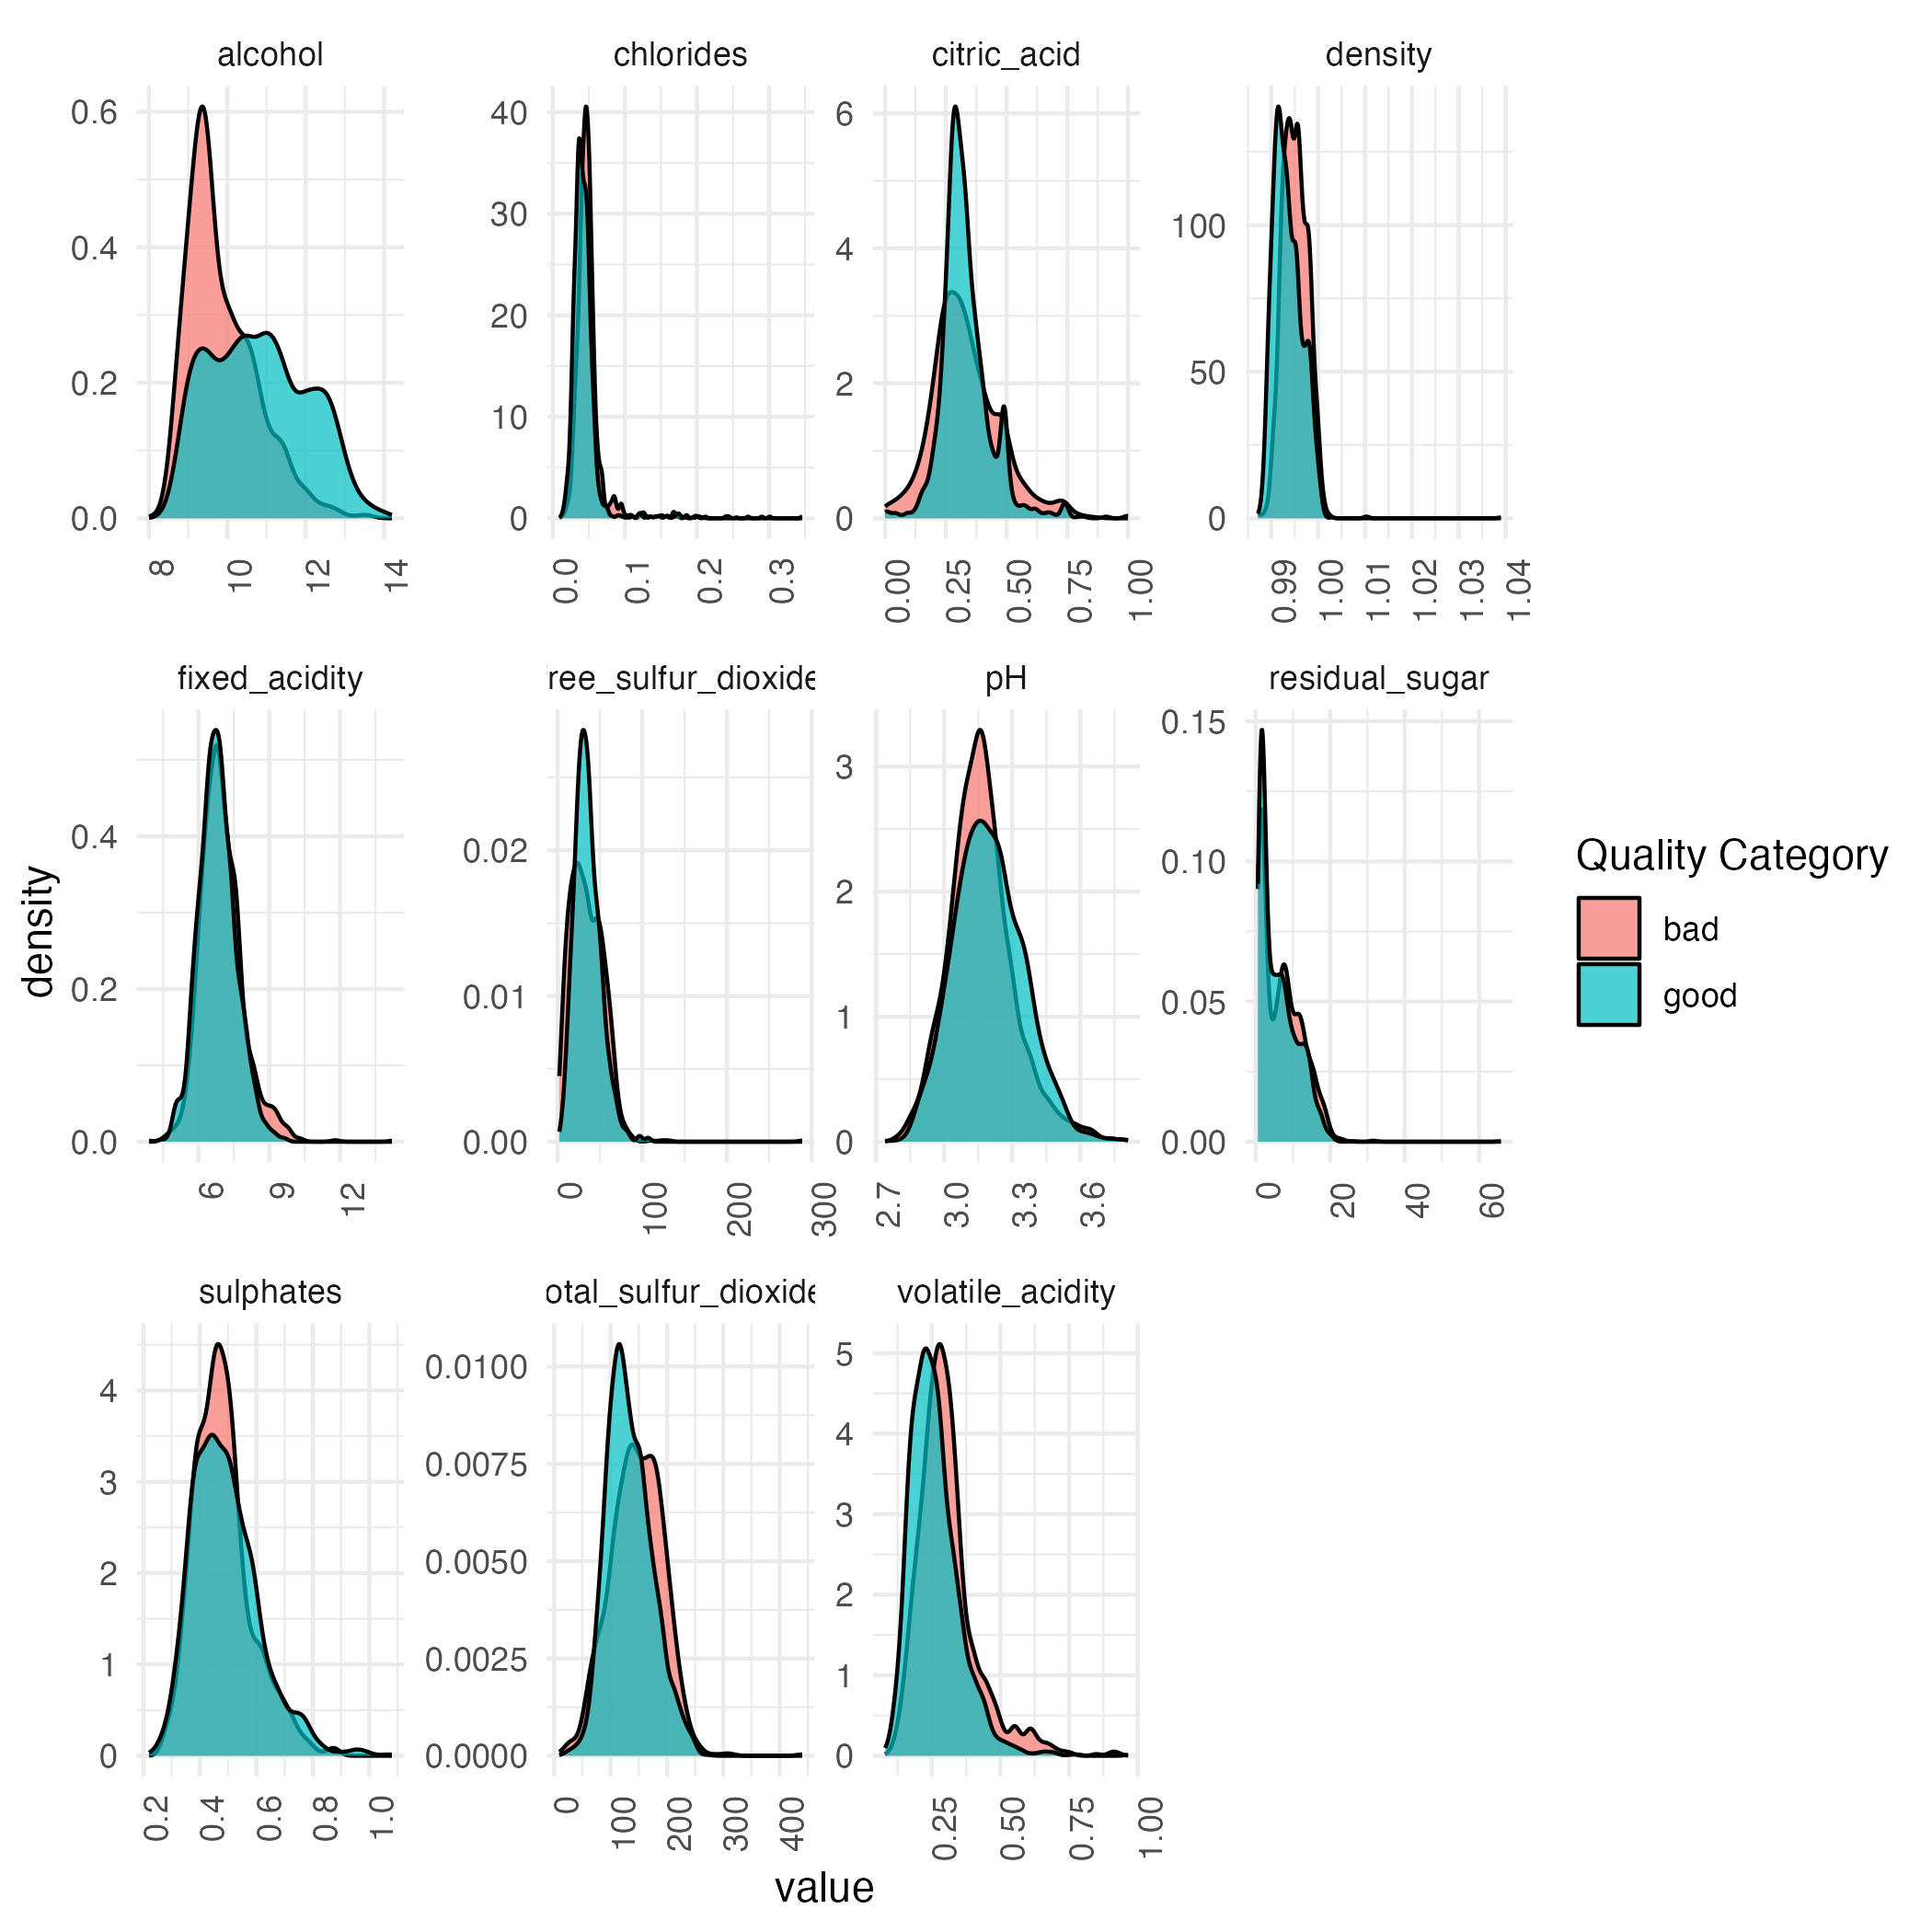
\includegraphics[width=0.9\textwidth,height=\textheight]{../results/03_feature_dist_plot.png}

}

\caption{\label{fig-feat-dist}Distributions of feature values between
both classes of wine.}

\end{figure}%

In the Figure~\ref{fig-feat-dist} above, alcohol, volatile acidity,
total sulfur dioxide content, density, chlorides, and residual sugar of
the wines all seem to have distinct distributions for both classes of
wine; the distributions have non-overlapping peaks and regions. Such
features are good to add in the model because they can be used to
identify one type of wine from the other.

Next, we perform hyperparamter optimization and make the train and fit
the model using cross-validation to find the optimal K value for this
classifier.

\begin{longtable}[]{@{}
  >{\raggedleft\arraybackslash}p{(\columnwidth - 12\tabcolsep) * \real{0.1333}}
  >{\raggedright\arraybackslash}p{(\columnwidth - 12\tabcolsep) * \real{0.1200}}
  >{\raggedright\arraybackslash}p{(\columnwidth - 12\tabcolsep) * \real{0.1467}}
  >{\raggedleft\arraybackslash}p{(\columnwidth - 12\tabcolsep) * \real{0.1333}}
  >{\raggedleft\arraybackslash}p{(\columnwidth - 12\tabcolsep) * \real{0.0400}}
  >{\raggedleft\arraybackslash}p{(\columnwidth - 12\tabcolsep) * \real{0.1333}}
  >{\raggedright\arraybackslash}p{(\columnwidth - 12\tabcolsep) * \real{0.2933}}@{}}

\caption{\label{tbl-cv-metrics}Cross-validations scores for different K
values}

\tabularnewline

\toprule\noalign{}
\begin{minipage}[b]{\linewidth}\raggedleft
neighbors
\end{minipage} & \begin{minipage}[b]{\linewidth}\raggedright
.metric
\end{minipage} & \begin{minipage}[b]{\linewidth}\raggedright
.estimator
\end{minipage} & \begin{minipage}[b]{\linewidth}\raggedleft
mean
\end{minipage} & \begin{minipage}[b]{\linewidth}\raggedleft
n
\end{minipage} & \begin{minipage}[b]{\linewidth}\raggedleft
std\_err
\end{minipage} & \begin{minipage}[b]{\linewidth}\raggedright
.config
\end{minipage} \\
\midrule\noalign{}
\endhead
\bottomrule\noalign{}
\endlastfoot
1 & accuracy & binary & 0.7710117 & 10 & 0.0064373 &
Preprocessor1\_Model01 \\
6 & accuracy & binary & 0.7678098 & 10 & 0.0064423 &
Preprocessor1\_Model02 \\
11 & accuracy & binary & 0.7683921 & 10 & 0.0051562 &
Preprocessor1\_Model03 \\
16 & accuracy & binary & 0.7689777 & 10 & 0.0055471 &
Preprocessor1\_Model04 \\
21 & accuracy & binary & 0.7730628 & 10 & 0.0055958 &
Preprocessor1\_Model05 \\
26 & accuracy & binary & 0.7707304 & 10 & 0.0061132 &
Preprocessor1\_Model06 \\

\end{longtable}

\begin{figure}

\centering{

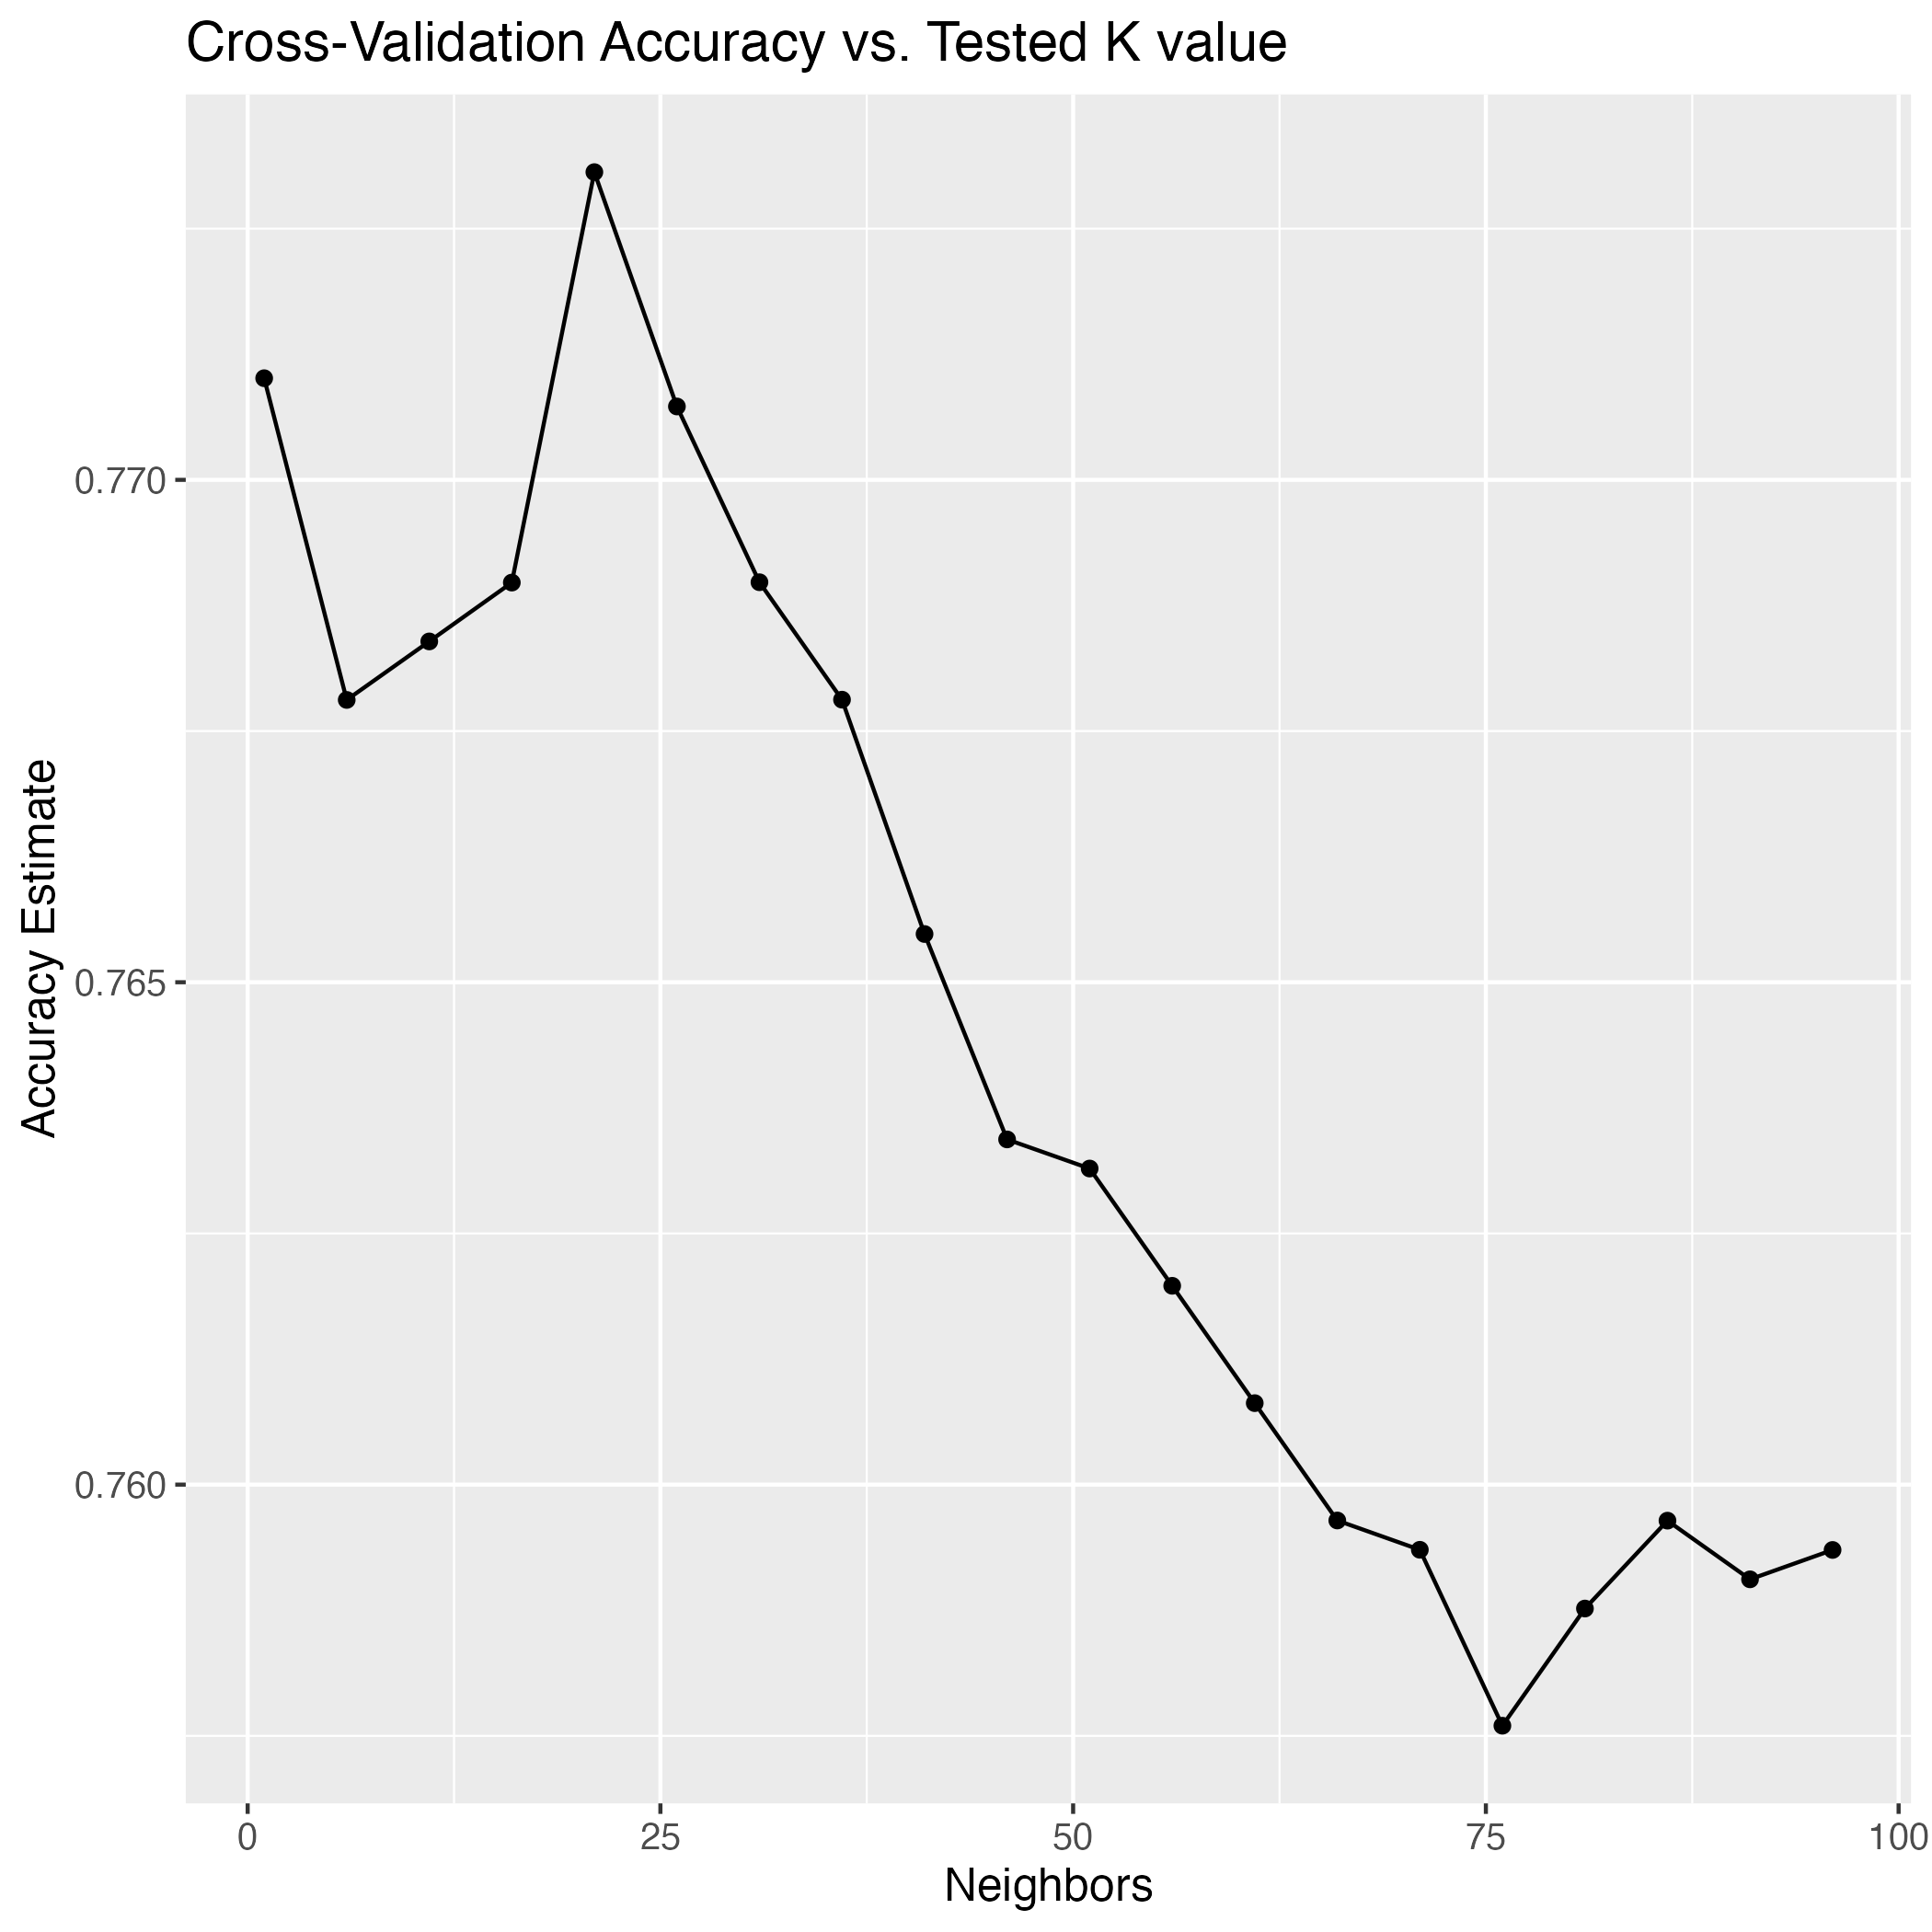
\includegraphics[width=0.9\textwidth,height=\textheight]{../results/06_accuracies_vs_k_plot.png}

}

\caption{\label{fig-acc-k}Accuracy scores for different values of K.}

\end{figure}%

Figure~\ref{fig-acc-k} shows us that as K becomes larger, the accuracy
of the model decreases. The model is overfitted at low K values and
tends toward underfitting as K increases. The ideal K value for this
problem seems to be around 20-25. Specifically, the best value for K is
21.

Finally, we use our test set to evaluate the classifier. We use several
metrics to assess our model as seen below.

\begin{longtable}[]{@{}llr@{}}

\caption{\label{tbl-test-acc}Accuracy and other metrics for evaluating
the model}

\tabularnewline

\toprule\noalign{}
.metric & .estimator & .estimate \\
\midrule\noalign{}
\endhead
\bottomrule\noalign{}
\endlastfoot
accuracy & binary & 0.7734694 \\
precision & binary & 0.7178082 \\
recall & binary & 0.5325203 \\

\end{longtable}

\begin{figure}

\centering{

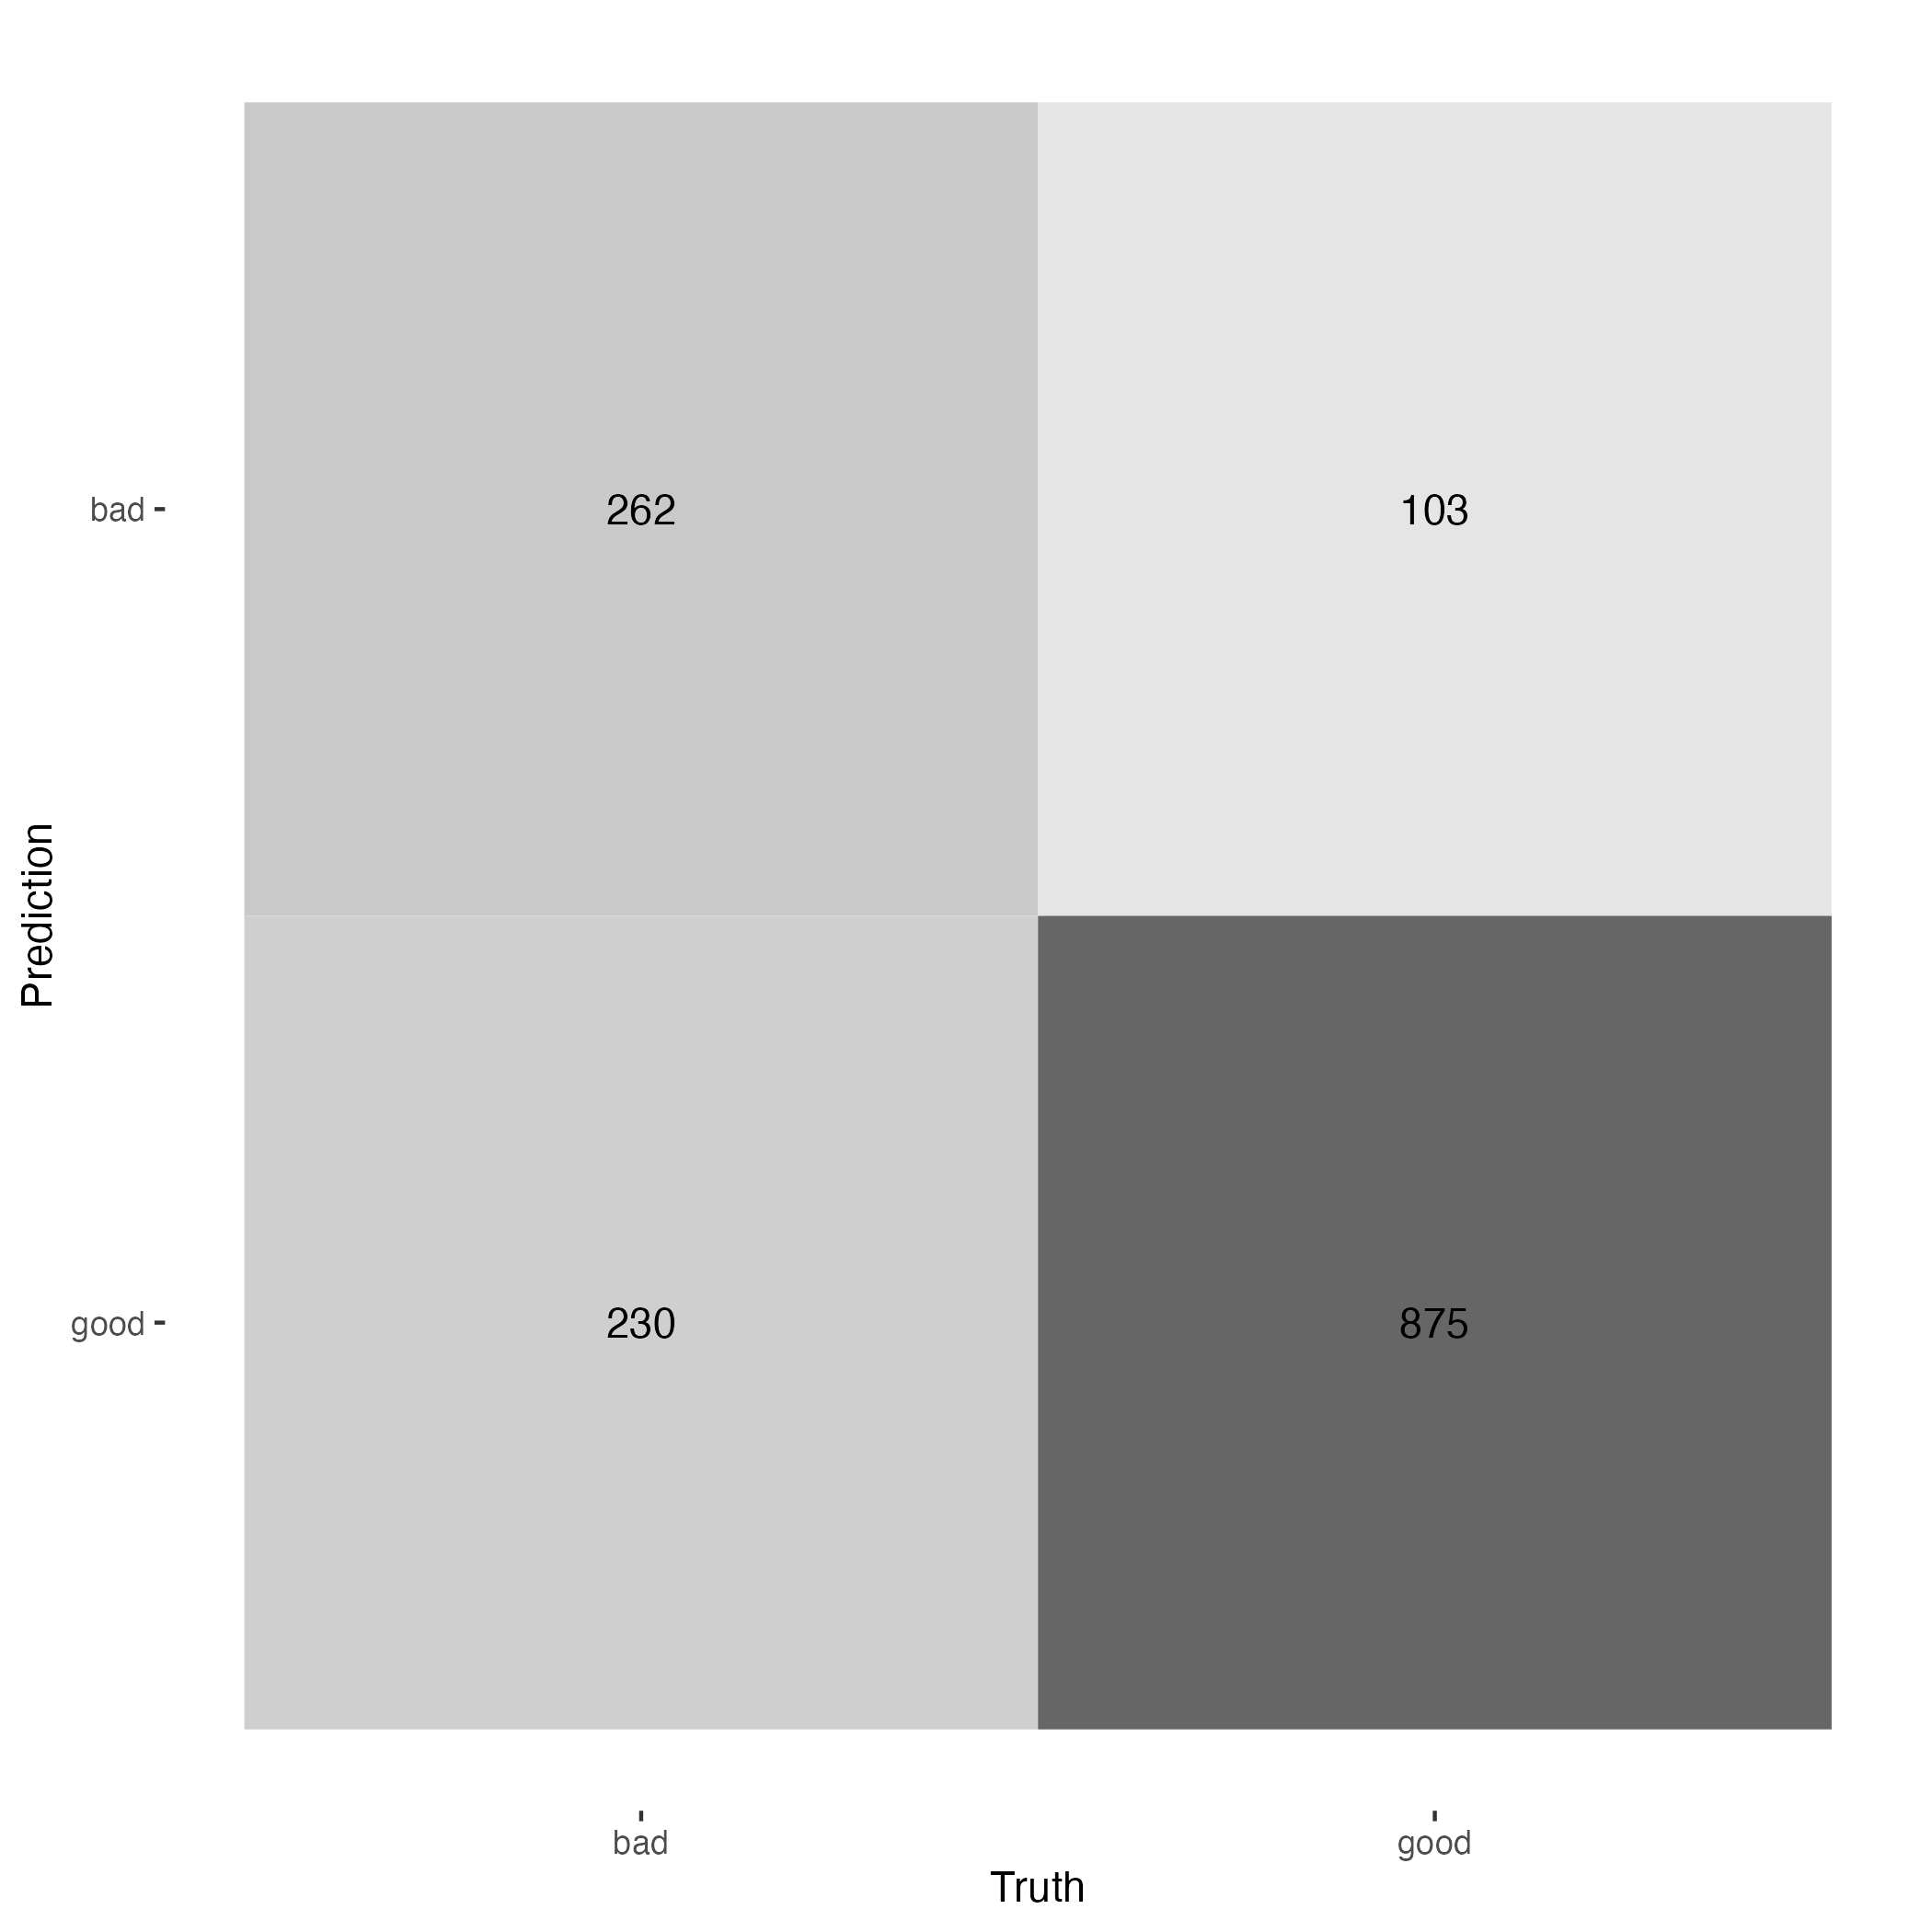
\includegraphics[width=0.7\textwidth,height=\textheight]{../results/09_confusion_matrix.png}

}

\caption{\label{fig-conf-mat}Confusion Matrix.}

\end{figure}%

Table~\ref{tbl-test-acc} above present the accuracy, precision, and
recall of our model on the test set. With an accuracy of 0.77, out model
is good but can clearly be improved upon. Additionally, for the recall
and precision tests, the good wine category is considered to be the
positive class. We can see that the recall is high, meaning that the
model has a high true positive rate (TPR). Figure~\ref{fig-conf-mat}
shows the confusion matrix, further emphasizing the model assessment.

\subsection{Discussion}\label{discussion}

The wine-quality prediction model seems to do okay with the test data,
having an accuracy of 0.77. It does a decent job at classifying good
wines as good, where \textasciitilde90\% of true good wines were
predicted to be good-quality. However, the model seems to not have a
high true negative rate; only \textasciitilde50\% of true bad wines were
predicted to be bad quality (as seen in Table~\ref{tbl-test-acc} and
Figure~\ref{fig-conf-mat}). We could try to increase the sensitivity of
the model or further optimize it, but seeing as wine quality tends to be
quite subjective and that the implications of an incorrect prediction
are not severe, this model is passable as a predictor. To improve this
model, we could use a more concrete and quantitative approach to feature
selection and choose a metric that is suited for a 1:2 class ratio
within the dataset. We could also use a different classification
strategy such as SVM or Random Forest Classifier. In its current state,
this model is best used as a reference where wine producers and
consumers can predict wine qualities while determining the quality
through other means as well.

\subsection*{References}\label{references}
\addcontentsline{toc}{subsection}{References}

\phantomsection\label{refs}
\begin{CSLReferences}{1}{0}
\bibitem[\citeproctext]{ref-repr}
Angerer, Philipp, Thomas Kluyver, and Jan Schulz. 2023. \emph{Repr:
Serializable Representations}.
\url{https://CRAN.R-project.org/package=repr}.

\bibitem[\citeproctext]{ref-wine_quality}
Cortez, Cerdeira, P., and J.. Reis. 2009. \emph{Wine Quality}. UCI
Machine Learning Repository. \url{https://doi.org/10.24432/C56S3T}.

\bibitem[\citeproctext]{ref-wine_relevant_atts}
Fernandes Ferreira Madureira, T.C., and F. J. Simões de Sousa Nunes.
2013. \emph{Relevant Attributes of Portuguese Wines: Matching Regions
and Consumer's Involvement Level}. International Journal of Wine
Business Research. \url{ttps://doi.org/10.1108/17511061311317318}.

\bibitem[\citeproctext]{ref-tidymodels}
Kuhn, Max, and Hadley Wickham. 2020. \emph{Tidymodels: A Collection of
Packages for Modeling and Machine Learning Using Tidyverse Principles.}
\url{https://www.tidymodels.org}.

\bibitem[\citeproctext]{ref-R}
R Core Team. 2019. \emph{R: A Language and Environment for Statistical
Computing}. Vienna, Austria: R Foundation for Statistical Computing.
\url{https://www.R-project.org/}.

\bibitem[\citeproctext]{ref-kknn}
Schliep, Klaus, and Klaus Hechenbichler. 2016. \emph{Kknn: Weighted
k-Nearest Neighbors}. \url{https://CRAN.R-project.org/package=kknn}.

\bibitem[\citeproctext]{ref-vinho_verde}
\emph{Vinho Verde}. 2024. CVRVV.
\url{https://www.vinhoverde.pt/en/homepage}.

\bibitem[\citeproctext]{ref-tidyverse}
Wickham, Hadley. 2017. \emph{Tidyverse: Easily Install and Load the
'Tidyverse'}. \url{https://CRAN.R-project.org/package=tidyverse}.

\bibitem[\citeproctext]{ref-psych}
William Revelle. 2024. \emph{Psych: Procedures for Psychological,
Psychometric, and Personality Research}. Evanston, Illinois:
Northwestern University. \url{https://CRAN.R-project.org/package=psych}.

\bibitem[\citeproctext]{ref-knitr}
Xie, Yihui. 2014. {``Knitr: A Comprehensive Tool for Reproducible
Research in {R}.''} In \emph{Implementing Reproducible Computational
Research}, edited by Victoria Stodden, Friedrich Leisch, and Roger D.
Peng. Chapman; Hall/CRC.
\url{http://www.crcpress.com/product/isbn/9781466561595}.

\end{CSLReferences}



\end{document}
